\section{Deep Learning and Neural Network}
\label{Chap:Mech:NN}

As previously mentioned in Chapter \ref{Chap:Mech:DFT}, \ac{DFT} calculations are accurate but also computationally costly. In order to solve the short time span of \ac{DFT} simulations, researchers fit \ac{DFT} results to classical force fields or empirical interatomic potentials, which are simpler analytical formulas or functional. Classical force fields or empirical interatomic potentials simplify the description of inter-atomic interactions by summing components of the short-ranged bonding\cite{jones1924determination}, angular\cite{justo1998interatomic}, dihedral\cite{cornell1995second}, and long-ranged Coulomb interaction\cite{liang2013classical}. Empirical potentials can be used in large-scale atomistic simulations with a reduced computational cost. Scientists and researchers have been constantly working on fitting more accurate empirical potentials to improve statistical sampling and accuracy of \ac{MD} and \ac{MC} simulations for the longer time domain. Due to the simplicity of analytical formulas and costly \ac{DFT} calculations, empirical potentials can only focus on a limited number of material properties of the fitted system. As the number of species included in the system increases, it is also more difficult to fit the desired empirical potential. Besides, empirical potentials are, in general, good at describing the interactions close to the equilibrium, but not very well at intermediate or transitional states. Therefore, to study the early nucleation stage of multi-component systems via vacancy diffusion, a more complex functional need to be used, which could be deep learning or \ac{NN} methods.

\begingroup
\begin{figure}[!ht]
  \centering
  \subfigure[]{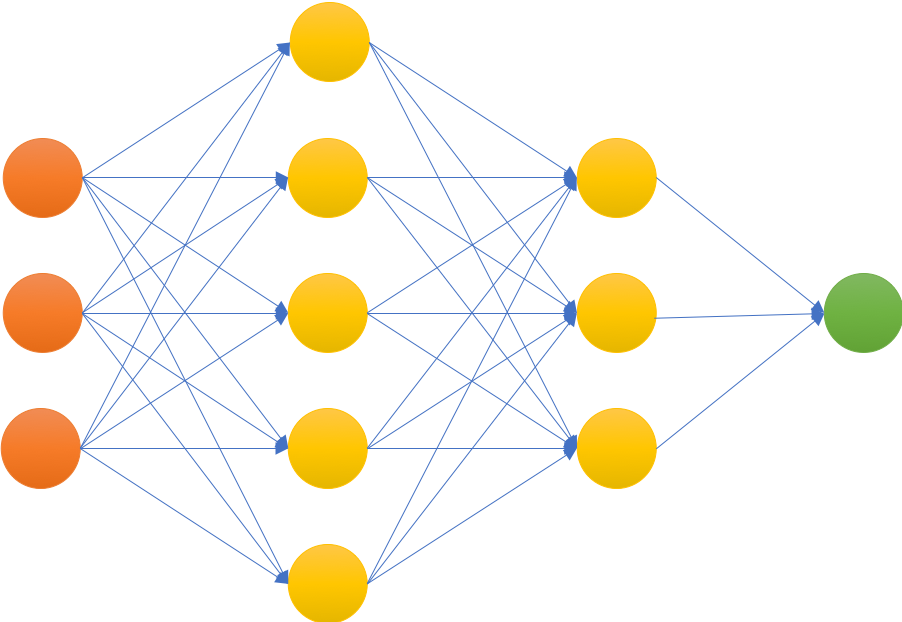
\includegraphics[width=0.9\linewidth]{Methods/plots/nn.png}}
  \caption[Illustration plot of a neural network.]{Illustration plot of a neural network. Orange, yellow, and green nodes indicate the input layer, hidden layers, and output, respectively.}
  \label{Chap:Meth:NN:fig1}
\end{figure}
\endgroup

Deep learning is a special category of machine learning models that uses a network of neurons, which are arranged in (fully/partially) interconnected layers. A \ac{NN} works similarly to the human brain’s neural connectivity, which will be activated under certain circumstances using various activation functions. \ac{NN}s are non-linear functions with parameters in different layers, called weights. Weights are optimizable through the back-propagation method of a cost function with respect to each weight. The input layer collects input patterns. The output layer has classifications or regression values to which input patterns are related. Hidden layers fine-tune the input weighting parameters until the \ac{NN}’s cost function is minimal. It is hypothesized that hidden layers extrapolate features in the input data that have predictive power about the outputs. In Figure \ref{Chap:Meth:NN:fig1}, a two-layer \ac{NN} is shown. Three orange nodes on the left indicate input nodes, which can be atom species encoding in the on-lattice bulk diffusion model. Yellow nodes in the middle are two layers of fully connected hidden layers. The green node on the right is the output layer, which can be the diffusion barrier. In practice, the neural network architecture will be much more complicated. Details of fitting diffusion barriers will be discussed in Chapter \ref{chap:Al/Vac}.